\documentclass[../report.tex]{subfiles}
%\graphicspath{{\subfix{../img/}}}

\begin{document}
\subsection{Time management}
We aimed to include everyone in all areas of the project deployment. This meant
we insured that everyone got the opportunity to be involved, with a task
fitting to there knowledge level.

We began with creating a general time plan for the whole semester project
progress.
\begin{figure}[H]
    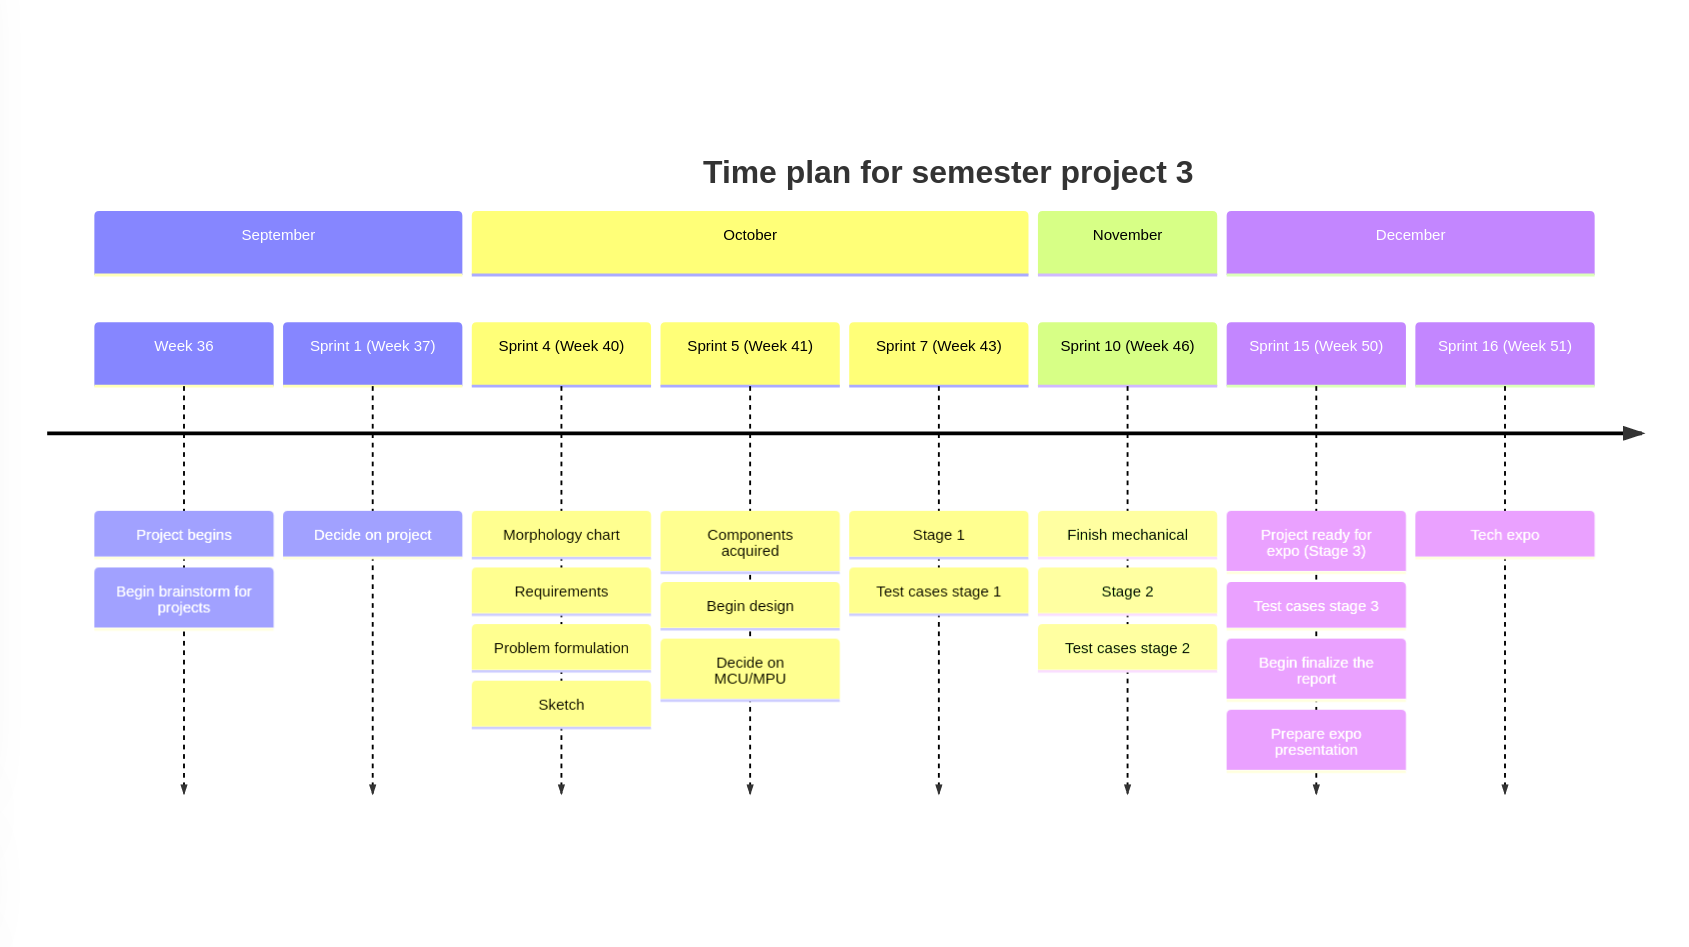
\includegraphics[width=\textwidth]{Management/timeplan.png}
    \caption{Initial time plan}
\end{figure}

\subsection{Task management}

We adopted the Scrum agile management framework and customized some parts of it to fit our project
and teams needs. We chose specifically this model due to the agile planing it introduces, and gradual
learning curve. We defined a sprint to be 7 days, from friday to friday with an estimate of 8 hours of
workload per team member. We categorized each task according to the time estimated to complete it
using these tags:

\begin{itemize}
    \item Sønderborg - 0.5 hours
    \item Keil - 1 hours
    \item Valencia - 2 hours
    \item Budapest - 4 hours
    \item Hamburg -  6 hours
\end{itemize}

We chose our home cities and sorted them by size to make it more simple to use
in conversations and to give a better visual idea of the task size. We decided
that the time limited on a task should be 6 hours. If a task would require more
time then it should be split into multiple tasks. This was to ensure that it
was possible to see if the task was possible to achieve before investing more
time into it.

\subsection{Individual evaluation}
A short evaluation of the project from each member in their own opinion. This is used to improve
upcoming projects, to prevent making the same mistakes again.
\textbf{member name:}
Write here
\textbf{member name:}
Write here
\textbf{member name:}
Write here
\textbf{member name:}
Write here
\textbf{member name:}
Write here
\textbf{member name:}
Write here
\end{document}